% !Mode:: "TeX:UTF-8"
%% This is file `mcmthesis-demo.tex',
%% generated with the docstrip utility.
%%
%% The original source files were:
%%
%% mcmthesis.dtx  (with options: `demo')
%%
%% -----------------------------------
%%
%% This is a generated file.
%%
%% Copyright (C)
%%     2010 -- 2015 by Zhaoli Wang
%%     2014 -- 2016 by Liam Huang
%%     2017         by Zhuang Ma
%%     2018美赛,为了迈思数模内部学员更快的掌握CTEX,由迈思数模站长对本模板进行调整
%% This work may be distributed and/or modified under the
%% conditions of the LaTeX Project Public License, either version 1.3
%% of this license or (at your option) any later version.
%% The latest version of this license is in
%%   http://www.latex-project.org/lppl.txt
%% and version 1.3 or later is part of all distributions of LaTeX
%% version 2005/12/01 or later.
%%
%% This work has the LPPL maintenance status `maintained'.
%%
%% The Current Maintainer of this work is Liam Huang.
%% 上述内容为介绍改模板的背景

\documentclass{mcmthesis}
\mcmsetup{CTeX = true,   % 使用 CTeX 套装时,设置为 true
        tcn = 84018, problem = C,
        sheet = true, titleinsheet = true, keywordsinsheet = true,
        titlepage = true, abstract = false}
%设置摘要页格式,一般按照该设置就行,true表示选择,false表示不选择,需要修改控制号和选择的题目
\usepackage{palatino}
\usepackage[section]{placeins}
%\usepackage{lipsum} %添加lipsum宏包,就是随机生成一段文本,可以不使用

\usepackage[UTF8, nocap]{ctex} %如果想使用中文输入的话,可以增加该宏包
\usepackage{amsmath}

\title{We Will Get O Prize(Not U Prize)}
%\author{\small \href{http://www.latexstudio.net/}
% {
\includegraphics[width=7cm]{mcmthesis-logo}}}
%\date{\today}

%正文摘要和控制页摘要名字修改
%\def\abstractname{Abstract}
%\def\sheetsummaryname{Summary}
\tolerance=1
\emergencystretch=\maxdimen
\hyphenpenalty=10000
\hbadness=10000


\begin{document}

 %控制页摘要内容
\begin{sheetsummary}
%\lipsum[1]
%lipsum是显示一段无意义的文字
%Ru guo ni bu xiang xian shi zhe duan wen zi, qing ba \textit{lipsum} shanchu.\\
%如果你不想显示上面的那段文字,那就把 \textit{lipsum}删掉
%获得更多的latex教材,请添加latex交流群,或者关注迈思数模微信公众号:shumohome
%并回复“LATEX资料”
%美赛LATEX模板交流群:193607493
hello world
\end{sheetsummary}

% %正文摘要内容
%\begin{abstract}
%\lipsum[2]
%\end{abstract}

%关键词
\begin{keywords}
hello; world
\end{keywords}

\maketitle
 % Generate the Table of Contents, if it's needed.
\tableofcontents
\newpage

\section{Overview}
    \subsection{Background}
    The rapid development of modern social economy benefits from the development of energy production. The issue of energy usage and production has always been the focus of world economic development.

    In the 21st century, with the economic development and improvement, the energy shortage and the increasing contradiction between supply and demand. Meanwhile, the production and use of fossil energy sources have had a huge negative impact on the environment. Therefore, developing clean and renewable energy is imperative.

    The differences between states such as geography, industry, population, climate lead to the contradiction of energy supply.
    Interstate cooperation and joint management and development of clean and renewable energy are regarded as the best solution to these problems. Nowadays four state governors  – California, Arizona, New Mexico and Texas  –  wish to form a realistic new energy compact. Texas leads the country in total (non-hydro) installed renewable energy capacity, almost all of which comes from the state’s 9,410 MW of wind capacity. California is the leader in solar energy installed capacity, both for photovoltaic technology (738 MW) and concentrating solar power (364 MW).

    \subsection{Restatement of the Problem}
    We are required to provide an overview of energy profile for each of the four states and model how these profiles have evolved from 1960 to 2009. In addition, it is necessary to make our results understandable through discussion, including similarities and differences between 4 states. Then we need to establish a criteria model and choose the "best" profile use of cleaner, renewable energy usage targets. Finally, we need to give our suggestions about exact action to achieve the goal we set based on what we predict.

    In order to determine whether it is clean and renewable energy, for which we check the information and classification of various types of energy.

    \noindent
    cleaner, renewable energy ( defination from SEDS and ):
    \begin{itemize}
      \item Conventional hydroelectric power
      \item Solar thermal direct use energy and photovoltaic electricity net generation
      \item Electricity produced by wind
      \item Wood and wood-derived fuels, biomass waste
      \item Fuel ethanol minus denaturant
    \end{itemize}

\section{Notations and Assumptions}
    \subsection{Assumptions and Justifications}
        \noindent
        We make the following basic assumptions in order to simplify the problem. Each of our assumptions is justified and is consistent with the basic fact.
        \begin{enumerate}
            \item \textbf{Ignore the external costs caused by power generation other than coal:}

              In 2005, the mean external damage of coal in the United States due to coal combustion was 3.2 cents/kWh, The external cost of natural gas power generation is 0.16 cents/kwh, which is actually almost entirely caused by coal-fired power. Also life-cycle CO2 emissions from nuclear, wind, biomass, and solar appear so small as to be negligible compared with those from fossil fuels.(information comes from the report "Hidden cost of energy unpriced consequences of energy production and use" )
            \item \textbf{The conversion between generation and consumption is 100\%, and the consumption is used to represent the amount of power generation to evaluate.}
            \item \textbf{Economic growth and energy development are stable. We ignore the impact of major external emergencies}
        \end{enumerate}
    \subsection{Notations}
         \begin{table}[!htbp]
            \centering
                \begin{tabular}{c|l}
                  \hline
                  Symbol & Meaning \\
                  \hline
                  n & the number of samples \\
                  p & the number of original indicators \\
                  k & the number of principal component \\
                  X & \{$x_{ij}$\} original data matrix (i = 1, 2,…, n ; j = 1,2,…,p ) \\
                  Z & \{$z_{ij}$\} standardization matrix with z-scores (i = 1, 2,…, n ; j = 1,2,…,p ) \\
                  U & \{$u_{ij}$\} partial covariance matrix (i = 1, 2,…, n ; j = 1,2,…,p ) \\
                  C & \{$c_{ij}$\} covariance matrix (j = 1,2,…,p ) \\
                  R & \{$r_{ij}$\} correlation matrix (j = 1,2,…,p ) \\
                  F & \{$f_{ij}$\} The eigenvectors matrix of Z (j = 1,2,…,p ) \\
                  Y & \{$y_{ij}$\} principal component matrix (i = 1, 2,…, n ; j = 1,2,…,k) \\
                  V & \{$v_{ij}$\} decision matrix (i = 1, 2,…, n ; j = 1,2,…,k) \\
                  $A^+$/$A^-$ & positive / negative ideal profile \\
                  $S_{i}^+$/$S_{i}^-$ & positive / negative ideal profile \\
                  $\lambda_{j}$ & the eigenvalues of Z (j=1,2,…,p) \\
                  $y_{i}$ & principal component \\
                  $C_{i}$ & the final performance score in TOPSIS method \\
                  kmo & the value of KMO test \\
                  p & autoregressive terms \\
                  d & differential times \\
                  q & average moving term \\
                  $y_{t}$ & the original data sequence \\
                  $y_{t}^{'}$ & smooth data sequence \\
                  $\hat{\rho_{k}}$ & the auto-correlation function \\
                  $\hat{\varphi_{kk}}$ & partial auto-correlation function \\
                  \hline
                \end{tabular}
           \caption{Abbreviation and Description}
         \end{table}


\section{Statement of Our Model}
    \subsection{Model Overview}
    Firstly, considering energy production and consumption, environmental impact, technology, economy, we extract 12 variables from 605 variables to get general energy profile of each state.

    In order to show the evolution of energy production, we construct a comprehensive evaluation index system for the level of cleaner, renewable energy development. We use the \textbf{Principal Component Analysis} method to carry out the correlation cluster analysis of the index. To make the similarities and differences between 4 states understandable, we use \textbf{TOPSIS} method to show our results.At the same time, we can get the extracted principal componment choosing the "best" profile from comprehensive evaluation results ranking.

    After determining the “best” profile, we use \textbf{ARIMA} method to predict the energy profile of each state, especially as we evaluate the cleaner, renewable energy development in the future.

    \subsection{Model Theory}
        \subsubsection{Principal Component Analysis Theory}
        The purpose of PCA is to use the idea of dimensionality reduction to convert multipleindicators into a few composite indicators. When using statistical methods to study multivariable problems, too many variables will increase the computational complexity and increase the complexity of analyzing the problems. We hope that in the process of quantitative analysis, fewer comprehensive variables are involved to make the results more Intuitive.

        The method can be summarized as follows:

        \begin{enumerate}
          \item \textbf{Organize the data set and normalization}
          Supposing that there are n samples, and each sample has P indicators, the original variable data X are arranged as a set of n data vectors with each representing a single grouped observation of the p variables, which as shown in formula
              \begin{table}[!hbpt]
                \centering
                { X } = $\begin{vmatrix} { x }_{ 1 }^{ T } \\ { x }_{ 2 }^{ T } \\ ... \\ { x }_{ n }^{ T } \end{vmatrix}$ = $\begin{vmatrix} { { x }_{ 11 } } & { x }_{ 12 } & ... & { x }_{ 1p } \\ { x }_{ 21 } & { x }_{ 22 } & ... & { x }_{ 2p } \\ ... & ... & ... & ... \\ { x }_{ n1 } & { x }_{ n2 } & ... & { x }_{ np } \end{vmatrix}$              \end{table}

              We choose zero-mean normalization to standardize the original data matrix.The standard score of a raw score xij is shown as formula

             \begin{table}[!hbpt]
               \centering
               $${ z }_{ ij }\quad =\quad \frac { { x }_{ ij }-\mu_{j}  }{ \sigma_{j}  }$$
             \end{table}

             where:
             $\mu_{j}$ is the mean of the row j .

             $\sigma_{j}$ is the standard deviation of the row j.


          \item \textbf{Determine the correlation between the indicators}
              Correlation test is a statistical test of how the variables are related and how relevant they are. Thus, it’s also the basis of principal component analysis. The Kaiser-MeyerOlkin (KMO) test method is used in this model. Correlation coefficient is a statistical indicator of the close relationship between the response variables, whose range of values between 1 to -1.

          \item \textbf{Calculate the number of principal component}
          The correlation coefficient matrix of standardization matrix is calculated by
          \begin{table}[!hbpt]
               \centering
               $$ C=\frac { { Z }^{ T }Z }{ n-1 }  $$
          \end{table}
          Calculate the eigvalue of Z and arrange in descending order.
          \begin{table}[!hbpt]
               \centering
               $$ |Z - \lambda E| = 0  $$
          \end{table}
          The cumulative contribution rate of top k factors is shown in formula.
          \begin{table}[!hbpt]
               \centering
               $$ { \alpha  }_{ (k) }=\frac { \sum _{ j\quad = 1 }^{ k }{ { \lambda  }_{ j } }  }{ \sum _{ j\quad =\quad 1 }^{ p }{ { \lambda  }_{ j } }  }   $$
          \end{table}
          The goal is to choose a value of k as small as possible while achieving a reasonably high value of ${\alpha}_{k}$ on a percentage basis. Generally, the value of $\alpha_{(k)}$should be more than 80\%.

          \item \textbf{Determine the scores of  principal components}

          The scores of principal components are calculate method is shown as formula.
               $$ y_m = F_m \times B (m=1,2,...,k)  $$
        \subsubsection{Technique for Order Preference by Similarity to Ideal Solution}
          TOPSIS is a method of compensatory aggregation that compares a set of alternatives by identifying weights for each criterion, normalizing scores for each criterion and calculating the geometric distance between each alternative and the ideal alternative, which is the best score in each criterion.
          The method is carried out as follows :
        \begin{enumerate}
          \item \textbf{Organize the data set and normalization}
          Construct normalized decision matrix. This step transforms various attribute dimensions into non-dimensional attributes, which allows comparisons across criteria.
          In our model, we use the principal component matrix calculated as formula(10) following.
            \begin{table}[!hbpt]
               \centering
               $$ { Y }=\begin{vmatrix} { y }_{ 1 } \\ { y }_{ 2 } \\ ... \\ { y }_{ n } \end{vmatrix}=\begin{vmatrix} { { y }_{ 11 } } & { y }_{ 12 } & ... & { y }_{ 1k } \\ { y }_{ 21 } & { y }_{ 22 } & ... & { y }_{ 2k } \\ ... & ... & ... & ... \\ { y }_{ n1 } & { y }_{ n2 } & ... & { y }_{ nk } \end{vmatrix} $$
             \end{table}
           \item
           \end{enumerate}

        \begin{enumerate}
          \item \textbf{Calculate the weighted normalized criteria matrix}
          We  use a set of weights from PCA for each criteria $w_{j}$. Multiply each column of the normalized decision matrix by its associated weight. An element of the new matrix is shown as formula(11)
            \begin{table}[!hbpt]
               \centering
               $$ v_{ij} = w_j y_{ij}, (i = 1,2,...,n; j=1,2,...,k) $$
             \end{table}
        where
            \begin{table}[!hbpt]
               \centering
               $$ { w  }_{ j }=\frac { { { \lambda  }_{ j } }  }{ \sum _{ j\quad =\quad 1 }^{ k }{ { \lambda  }_{ j } }  } ,(j =1,2,...,k) $$
             \end{table}
            \item
           \end{enumerate}

        \begin{enumerate}
          \item \textbf{Determine the ideal and negative ideal profiles}
          Positive ideal solution is determined as formula(13)
            \begin{table}[!hbpt]
               \centering
               $$ { A }^{ + }=\{ { v }_{ 1 }^{ + },{ v }_{ 2 }^{ + },...,{ v }_{ k }^{ + }\}  $$
             \end{table}
        where
            \begin{table}[!hbpt]
               \centering
               $$ { v }_{ j }^{ + }=\{ max({ v }_{ ij }),if\quad j\in J_+;min({ v }_{ ij }),if\quad j\in J_-\}  $$
             \end{table}
        Negative ideal solution is determined as formula(15)
            \begin{table}[!hbpt]
               \centering
               $$ { A }^{ - }=\{ { v }_{ 1 }^{ - },{ v }_{ 2 }^{ - },...,{ v }_{ k }^{ - }\}  $$
             \end{table}
        where
            \begin{table}[!hbpt]
               \centering
               $$ { v }_{ j }^{ - }=\{ min({ v }_{ ij }),if\quad j\in J_+;max({ v }_{ ij }),if\quad j\in J_-\}   $$
             \end{table}
            \item
           \end{enumerate}

        \begin{enumerate}
          \item \textbf{Calculate the separation measures for each alternative}
         The separation from the positive ideal alternative is shown as formula(17):
            \begin{table}[!hbpt]
               \centering
               $$ { S }_{ i }^{ + }=\sqrt { \sum _{ j\quad =1 }^{ k }{ { ({ v }_{ ij }-{ v }_{ j }^{ + }) }^{ 2 } }  } ,i = 1,2,..n $$
             \end{table}
          The separation from the negative ideal alternative is shown as formula(18):
            \begin{table}[!hbpt]
               \centering
               $$ { S }_{ i }^{ - }=\sqrt { \sum _{ j\quad =1 }^{ k }{ { ({ v }_{ ij }-{ v }_{ j }^{ - }) }^{ 2 } }  } ,i = 1,2,..n $$
             \end{table}
            \item
           \end{enumerate}

        \begin{enumerate}
          \item \textbf{Calculate the relative closeness to the ideal profile}
         Calculate the similarity to the worst condition as formula(19):
            \begin{table}[!hbpt]
               \centering
               $$ C_{ { i } }=\frac { { S }_{ i }^{ - } }{ { S }_{ i }^{ + }+{ S }_{ i }^{ - } }  $$
             \end{table}
         where
         if $$ C_{i}=1 $$,the alternative sample has the best condition; and
         if $$ C_{i}=0 $$,the alternative sample has the worst condition.

            \item
           \end{enumerate}

        \begin{enumerate}
          \item \textbf{Rank the preference order}
        Rank the alternatives using $C_i$ index value in decreasing order. An alternative with largest index value ($C_i$) has shortest distance from positive ideal profile and farthest distance from negative ideal profile.

            \item
           \end{enumerate}

\section{Model Implementation and Results}
        \subsection{Energy Profile}

        \begin{enumerate}
          \item \textbf{Data extraction}
            To evaluate the performance of the energy profile (especially in C-R energy) for each states, we set 5 second grade indices , including energy supply, energy consumption, efficiency, Additional costs and C-R energy development prospects. On the basis of the second grade indicators, we set 10 third grade indices, including the total energy production, C-R energy production, C-R energy consumption ratio, C-R energy increase speed etc. The following table shows the index system for energy profile.

            \begin{figure}
              \centering
              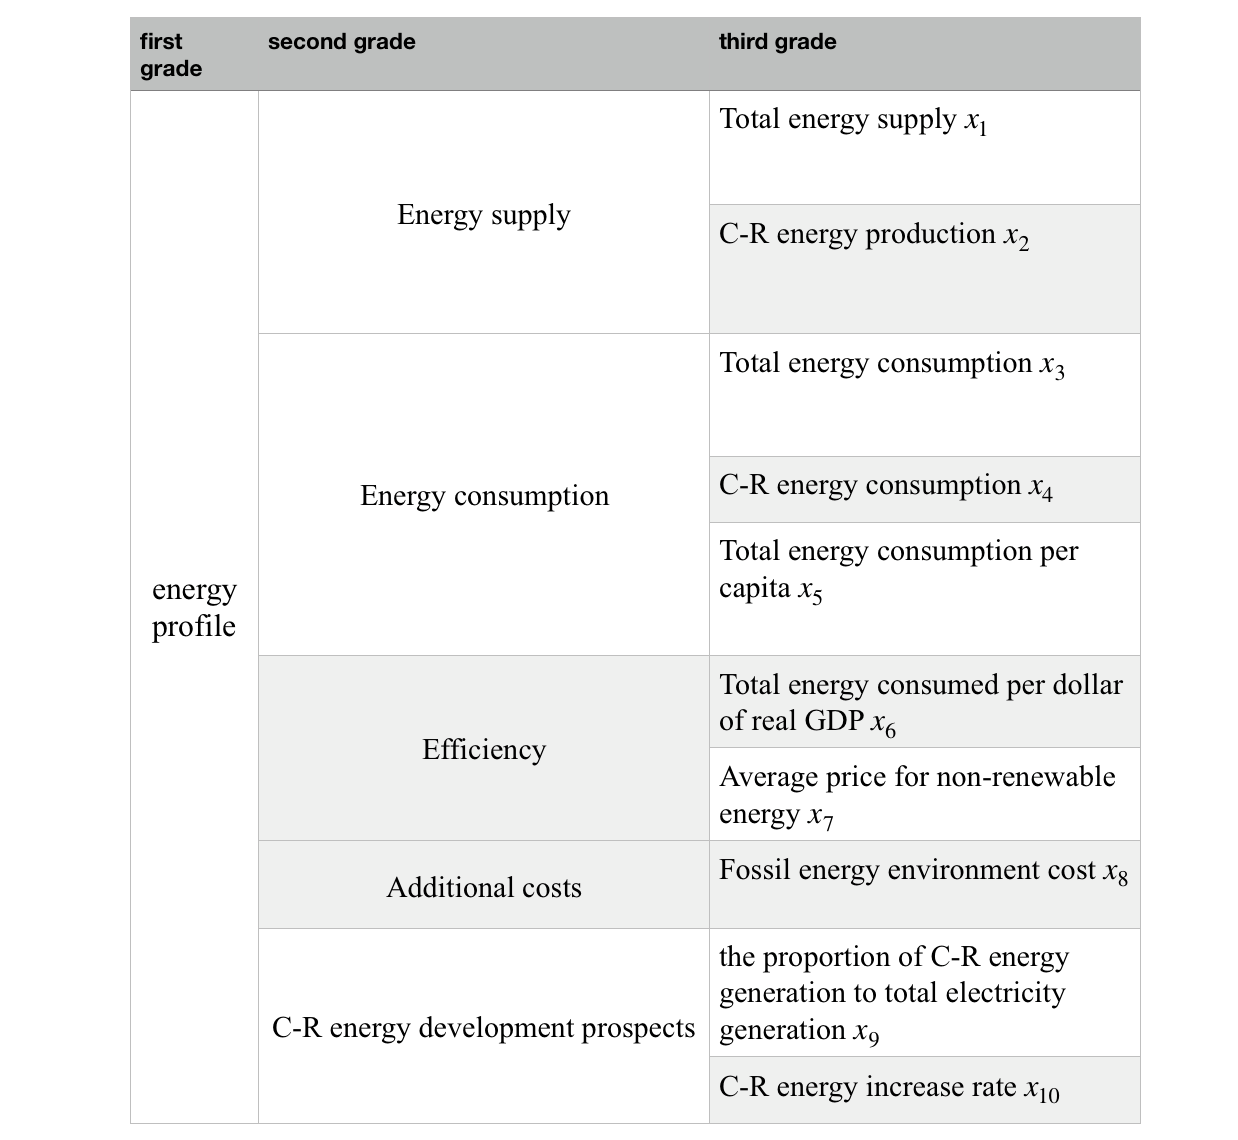
\includegraphics[width=400px]{ener.png}
            \end{figure}

        \item Note:The data comes from State Energy Data System (SEDS) Complete Dataset (All 50 states) (https://catalog.data.gov/dataset/state-energy-data-system-seds-complete-dataset-through- 2009\#sec-dates)
        \item Energy supply:the energy supply indicators are the most intuitive indicators showing the level of energy production and clean energy development in the region.
        \item Energy consumption: the energy consumption indicators truly reflect the use of energy in each state. Total energy consumption and total energy consumption per capita show us the demand of energy. C-R energy consumption
        \item Efficiency of energy utilization: the efficiency indicators describe energy production in technical aspect, which are the key factors that affect the development and utilization of  energy.
        \item Additional cost: the indicator directly reflect the effect of energy profile evaluation. It is measured mainly by the total amount of pollutants emitted from fossil energy. Compared to traditional fossil fuels, the application of clean energy can greatly reduce pollutant emissions.
        \item C-R energy development prospects: the prospect is characterized by C-R energy increase rate, the proportion of C-R energy generation to total electricity generation.
        We extract the average of last 5 years(2005-2009) and use the rank radar chart to indicate the energy profile of each state in each dimension.(exact data is given in the appendix). In addition, considering the purpose of 4 states, we will also analyze main energy usage proportion.
        \end{enumerate}

        \begin{enumerate}
          \item \textbf{Energy profile of each state}

          \item Arizona:
        \begin{figure}
            \centering
            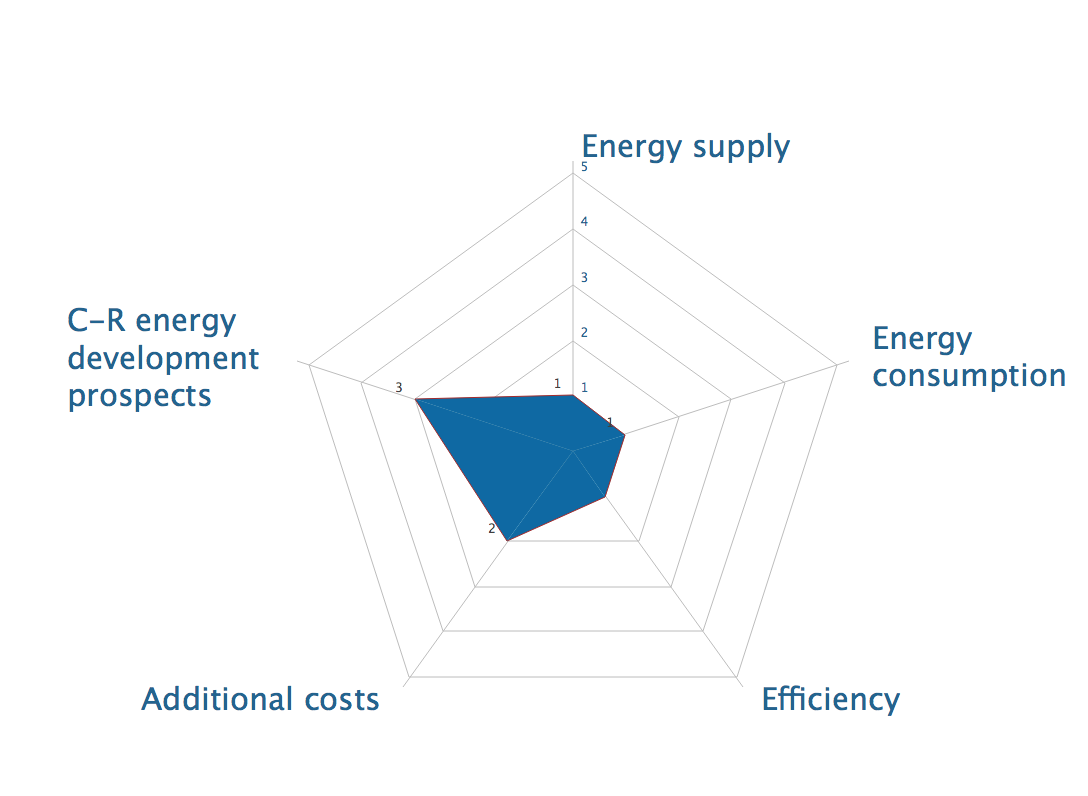
\includegraphics[scale=0.6]{AZ.png}
            \caption{Energy profile of Arizona}
        \end{figure}

        \begin{figure}[ht]
         \centering
         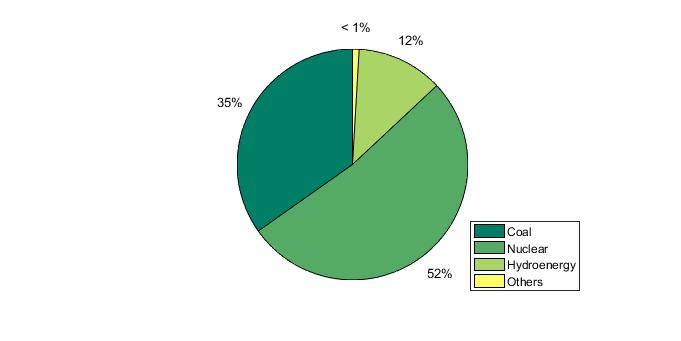
\includegraphics[scale=0.6]{AZ1.jpg}
         \caption{Energy proportion of Arizona}
        \end{figure}
     Arizona has few energy production and energy consumption, but it does have abundant Nuclear and hydroenergy potential. The state’s production utilization efficiency is low but with higher additional costs.
    \item California:
    \begin{figure}[ht]
    \centering
    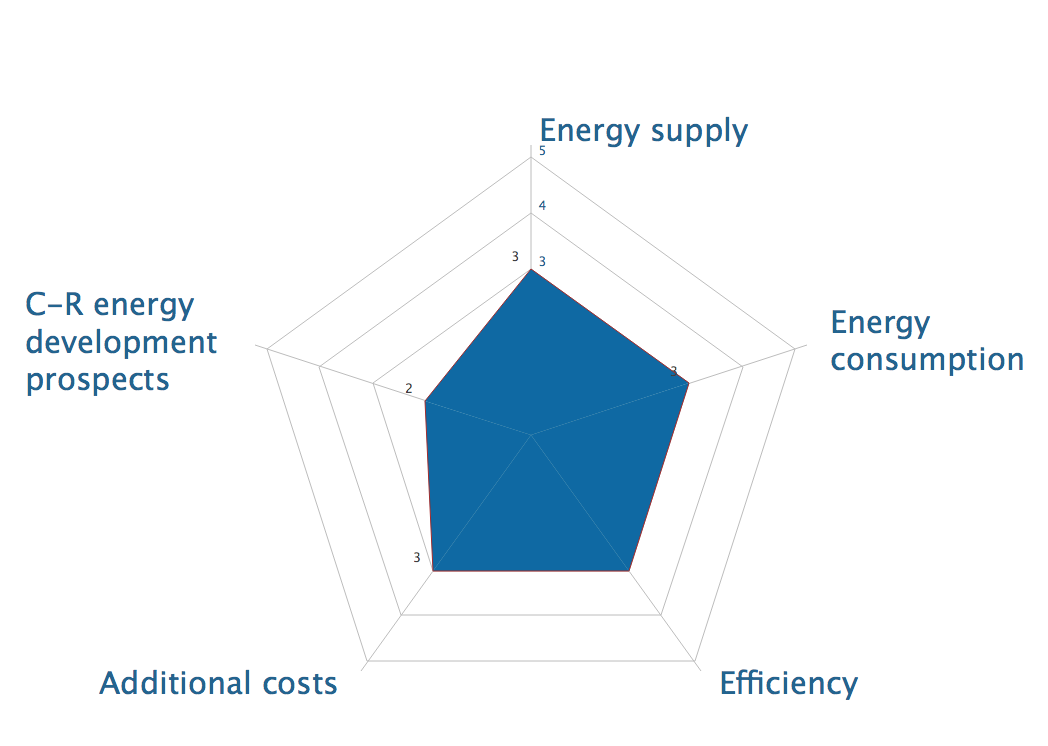
\includegraphics[scale=0.6]{CA.png}
    \caption{Energy profile of California}
    \end{figure}
    \begin{figure}[ht]
    \centering
    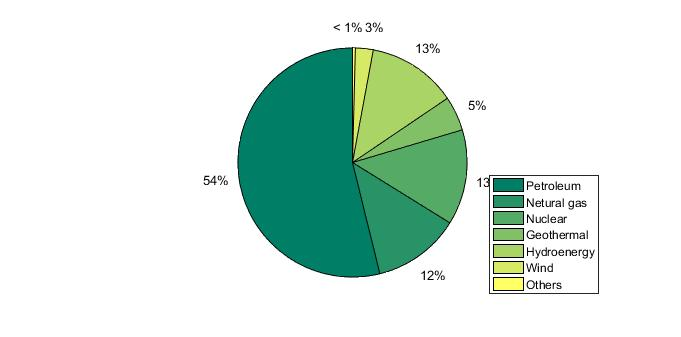
\includegraphics[scale=0.6]{CA1.jpg}
    \caption{Energy proportion of California}
    \end{figure}
     California’s total energy supply and demand is high, and all indictors are basically in a state of balance. California is also rich in energy resources. The state has an abundant supply of cleaner, renewable energy, including nuclear, Geothermal, wind etc.
    \item New Mexico:
    \begin{figure}[ht]
    \centering
    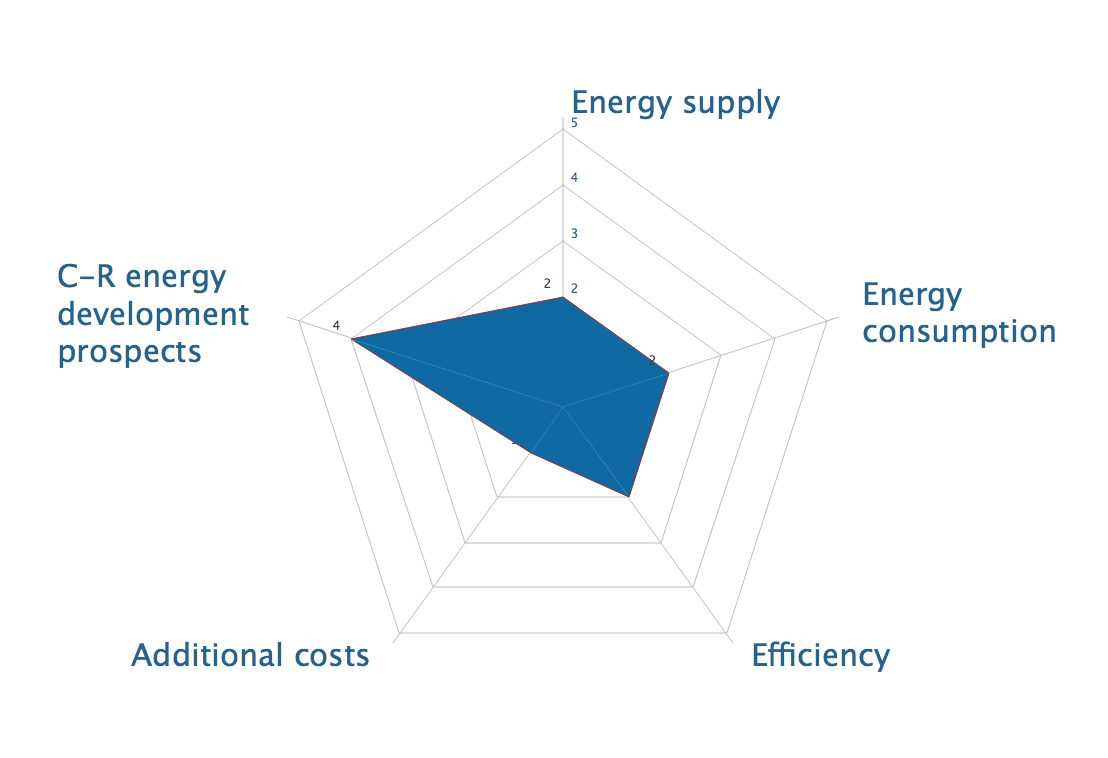
\includegraphics[scale=0.6]{NM.png}
    \caption{Energy profile of New Mexico}
    \end{figure}
    \begin{figure}[ht]
    \centering
    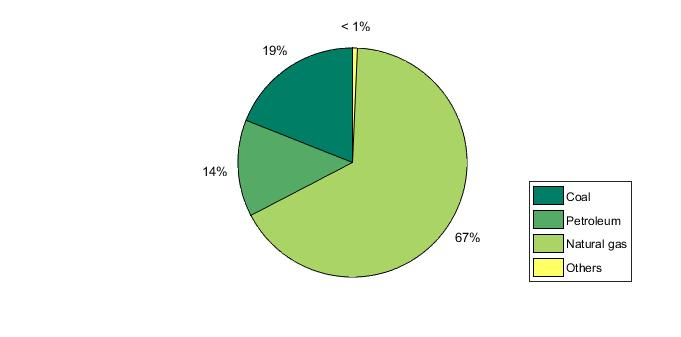
\includegraphics[scale=0.6]{NM1.jpg}
    \caption{Energy proportion of New Mexico}
    \end{figure}
     Though New Mexico uses fossil fuels to supply energy demand, it still does well in environment protection. Besides that, the state contains a wealth of fossil fuel and has abundant energy potential.
    \item Texas:

    \begin{figure}
      \centering
      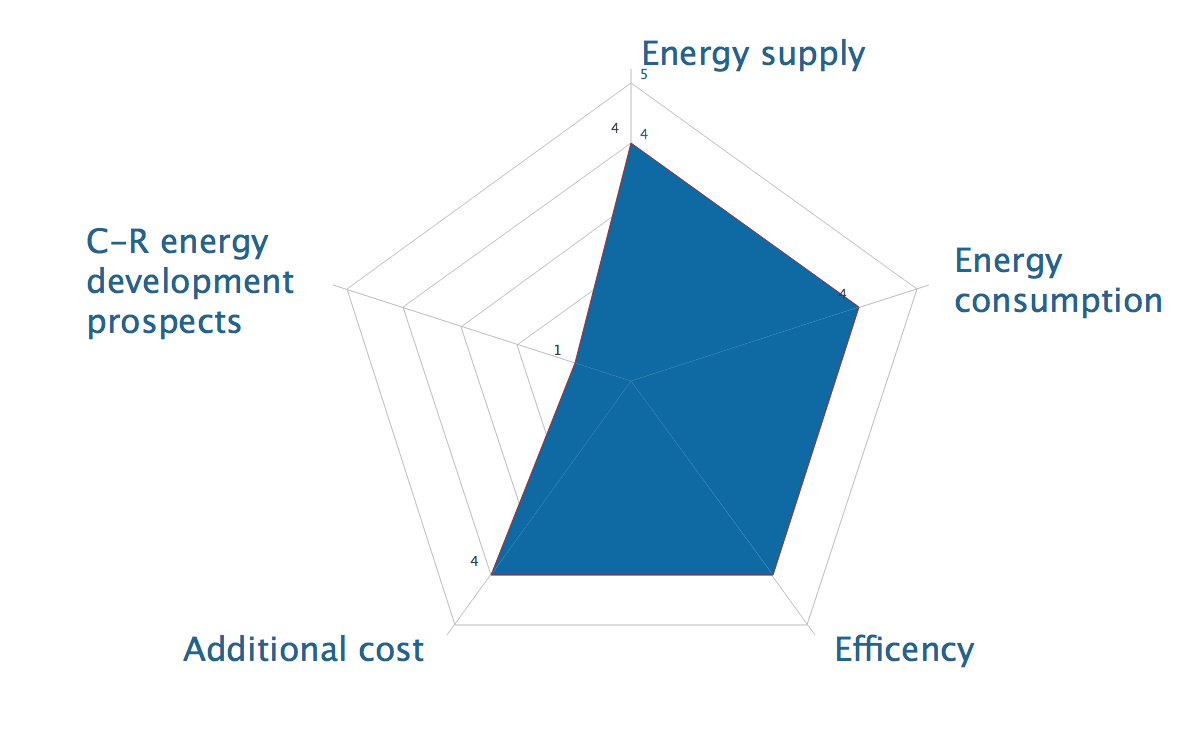
\includegraphics[scale=0.6]{TX.png}
      \caption{Energy profile of Texas}
    \end{figure}


    \begin{figure}
      \centering
      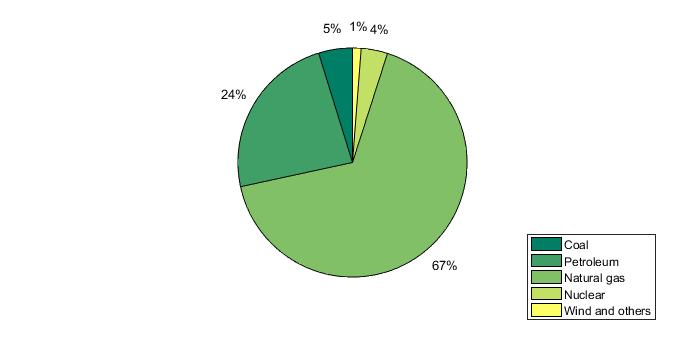
\includegraphics[scale=0.6]{TX1.jpg}
      \caption{Energy proportion of Texas}
    \end{figure}


     Texas has highest energy production, consumption and production utilization efficiency. And Texas is a large state with a wealth of energy resources. However, high environment damage and negative prospect of C-R energy development is considerable.
            \item
           \end{enumerate}


        \subsection{Evolution model}
        \begin{enumerate}
          \item \textbf{Determine the linear equation of principal components}
        Firstly, we extract principal components from 10 indicators. We use the average of last 5 years as a training set to determine the linear combination equations between principal components and evaluation index system.
      The indicators are as following:
      \begin{table}
      \begin{tabular}{|c|}
      \hline
      {Total energy supply $x_1$}\\
      \hline
      {C-R energy production $x_2$}\\
      \hline
      {The proportion of C-R energy generation to total electricity generation $x_3$}\\
      \hline
      { Average price for non-renewable energy $x_4$}\\
      \hline
      { Total energy consumption $x_5$}\\
      \hline
      { C-R energy consumption $x_6$}\\
      \hline
      { Total energy consumption per capita $x_7$}\\
      \hline
      {  Fossil energy environment cost $x_8$}\\
      \hline
      { Total energy consumed per dollar of GDP $x_9$}\\
      \hline
      {renewable energy increase rate $x_{10}$}\\
      \hline
      \end{tabular}
      \caption{indictors of evaluation system}

      \end{table}



      Through the standard processing of these data, the relative value of each index is obtained, as shown in table 1.

      \begin{table}
      \begin{tabular}{|c|c|c|c|c|c|c|c|c|c|c|}
      \hline
      { }&x1&x2&x3&x4&x5&x6&x7&x8&x9&x10\\
      \hline
      {AZ}&-0.7767&-0.5675&0.5419&-1.0061&-0.7565&-0.6559&-0.7178&-0.2267&-0.5546&-0.7450\\
      \hline
      {CA}&-0.3178&1.4478&1.0651&1.3715&0.5125&1.4381&-0.8089&-0.8225&-1.1043&-0.9622\\
      \hline
      {NM}&-0.3737&-0.7518&-0.4292&-0.3243&-0.9112&-0.7760&-0.4032&-0.4032&-0.6093&-1.0293\\
      \hline
      {TX}&1.4683&-0.1284&-1.1779&-0.0411&1.1553&-0.0963&1.14524&1.14524&1.0496&0.6780\\
      \hline
      \end{tabular}
      \caption{Standardized results of index data for 4 states}
      \end{table}
      Based on the standard data, we use the KOM test, and the value is 0.9145. So these data is very suitable for Principal Component Analysis.The coefficient matrix is shown in Appendix.

      The characteristic values of the correlation coefficient matrix are calculated. According to the calculation results, the last three principal components are listed in Table 3, since the characteristic value of the seventh principal component approaches zero. The characteristic values of principal components and the contribution rate of variance of the index system are shown in Table 3. In this study, the characteristic values of the last three principal components are larger, that is, the last three principal components contribute the most to the explanatory variables. Therefore, the extraction of the Last three principal components is the most appropriate and the cumulative variance contribution rate is 99$\%$, which combines most of the information on the level of clean energy development.
      \begin{table}
      \begin{tabular}{|c|c|c|c|}
      \hline
      { components }&{Total}&{Variance}&{Cumulative Variance}\\
      \hline
      {y1}&0.6468&6.468$\%$&6.468$\%$\\
      \hline
      {y2}&3.4019&34.019$\%$ & 40.487$\%$\\
      \hline
      {y3}&5.9513&59.913$\%$ & 99.999$\%$\\
      \hline
      \end{tabular}
      \caption{Eigenvalue and contribution rate of variance of the principal components}
      \end{table}
        The feature vectors of each principal component are calculated according to the matrix and the characteristic values, as shown in Table 4. Table 4 shows the expression of the three principal components y1, y2, y3.

        The linear combination equations between principal components and evaluation index system are shown as formulas.

          \begin{table}[!hbpt]
               \centering
               $${ y }_{ 1 }={ \begin{bmatrix} -0.1372 \\ 0.1066 \\ 0.1069 \\ 0.4970 \\ -0.2475 \\ 0.0866 \\ 0.0724 \\ -0.4721 \\ 0.2208 \\ 0.6065 \end{bmatrix} }^{ T }\begin{bmatrix} x_{ 1 } \\ x_{ 2 } \\ x_{ 3 } \\ x_{ 4 } \\ x_{ 5 } \\ x_{ 6 } \\ x_{ 7 } \\ x_{ 8 } \\ x_{ 9 } \\ x_{ 10 } \end{bmatrix}$$
              $${ y }_{ 2 }={ \begin{bmatrix} -0.3741 \\ -0.4014 \\ 0.0610 \\ -0.4187 \\ -0.5216 \\ -0.4082 \\ -0.1901 \\ -0.2053 \\ 0.0112 \\ 0.0538 \end{bmatrix} }^{ T }\begin{bmatrix} x_{ 1 } \\ x_{ 2 } \\ x_{ 3 } \\ x_{ 4 } \\ x_{ 5 } \\ x_{ 6 } \\ x_{ 7 } \\ x_{ 8 } \\ x_{ 9 } \\ x_{ 10 } \end{bmatrix}$$
          $${ y }_{ 3 }={ \begin{bmatrix} 0.2932 \\ -0.2733 \\ -0.4058 \\ -0.2024 \\ 0.0773 \\ -0.2683 \\0.3832 \\ 0.3460 \\ 0.4033 \\ 0.3557 \end{bmatrix} }^{ T }\begin{bmatrix} x_{ 1 } \\ x_{ 2 } \\ x_{ 3 } \\ x_{ 4 } \\ x_{ 5 } \\ x_{ 6 } \\ x_{ 7 } \\ x_{ 8 } \\ x_{ 9 } \\ x_{ 10 } \end{bmatrix}$$
             \end{table}
            It can be seen from the above expressions that the variance contribution rate of the principal , component y3 is 59.513$\%$. Total energy consumption, fossil energy environment cost and renewable energy consumption ratio and other five indices accounted for a larger proportion in the main component y3, so the main component y3 mainly reflects \textbf{the cost for energy}.

            The variance contribution rate of principal component y2 is 34.019$\%$.  Total energy consumed per dollar of real GDP, total energy consumption per capita and total energy consumed per dollar of real GDP in the main component of y2 is relatively large, so the main component of y2 mainly reflects \textbf{the degree for renewable energy exploit}.

            The variance contribution rate of principal component y1 is 6.468$\%$, which mainly reflects \textbf{the tendency of the renewable energy use}.
        \end{enumerate}

\subsection{"best" profile}

       Our goal is to determine the "best" profile of C-R energy use.From PCA analysis, we can conclude that $y_{1}$, $y_{2}$ associated with the criteria having a positive impact, and $y_{3}$associated with the criteria having a negative  impact.
      TOPSIS method is applied to rank the four sates in usage of C-R energy. The priority weights of states with respect to criteria, calculated by PCA can be used in TOPSIS. The weighted normalized decision matrix can be seen from table.

      \begin{table}
      \centering
      \begin{tabular}{cccc}
      \hline
      {}&{y1}&{y2}&{y3}\\
      \hline
      {AZ}&-0.800&\textbf{1.853}&-1.100\\
      \hline
      {CA}&\textbf{1.106}&-1.636&\textbf{-1.736}\\
      \hline
      {NM}&0.2707&1.559&0.405\\
      \hline
      {TX}&-0.5759&-1.177&2.431\\
      \hline
      \end{tabular}
      \caption{The weighted normalized decision matrix}
      \end{table}

      Then, using TOPSIS method, the ranking of sates are calculated. Table shows the evaluation results and final ranking of energy profiles for usage of C-R energy.

      \begin{table}
      \begin{tabular}{ccc}
      \hline
      {States}&{$C_i$}&{Ranking}\\
      \hline
      {AZ}&0.554&3\\
      \hline
      {CA}&0.443&4\\
      \hline
      \textbf{NM}&\textbf{0.687}&\textbf{1}\\
      \hline
      {TX}&0.597&2\\
      \hline

      \end{tabular}
      \caption{The final evaluation and ranking of states}
      \end{table}

      The "best" profile for use of C-R energy  belongs to New Mexico.



        \subsubsection{Autoregressive Integrated Moving Average Model}
        The basic idea of this ARIMA model is to assume that the time series under study is a non-stationary time series generated by a random process. The non-stationary time series is treated several times to make it a stationary time series. Then the time series observations Value to establish the autoregressive moving average model of the stochastic process, using the optimal model established to predict.ARIMA model has 3 parameters. It is usually recorded as ARIMA(p,d,q). ARIMA is one of ARMA's expansion.
        ARMA's general expression is as followed:
        $$y_{t}=\varphi_{1}y_{t-1}+\varphi_{2}y_{t-2}+...\varphi_{p}y_{t-p}+u_{t}$$
        \textbf{Predictive model establishment process:}
        \begin{enumerate}
          \item Obtain and pretreate the data:

           Do run-length test to determine whether the sequence is a smooth sequence. if it is a non-stationary sequence, using the difference method to make it smooth: $y_{t-i}^{'}$ = $y_{t}$ - $y_{t-1}$, The sequence is preprocessed. After each difference, the data is run-tested until the difference data can pass the stationarity test and recorded as d-difference to obtain a new stationary sequence: $y_{1}^{'}$, $y_{2}^{'}$, $y_{3}^{'}$.

          \item ARMA model recognition:

          Model recognition was performed by calculating the(ACF)$\hat{\rho_{k}}$and pre-processed (PACF)$\hat{\varphi_{kk}}$ of the preconditioned sequence $y_{t}^{'}$.

          $$\hat{\rho_{k}} = \frac{\sum_{t=1}^{N-k}y_{t+k}^{'}y_{t}^{'}}{N}$$

          $$\hat{\varphi}_{11} = \hat{\rho_{1}}$$
          $$\hat{\varphi}_{k+1,k-1} = (\hat{\rho}_{k+1}-\sum_{j=1}^{k}\hat{\rho}_{k+1-j}\hat{\varphi}_{kj})(1-\sum_{j=1}^{k}\hat{\rho}_{j}\hat{\varphi}_{kj})^{-1}$$
          $$\hat{\varphi}_{k+1,j} = \hat{\varphi}_{jk} - \hat{\varphi}_{k+1,k+1}\hat{\varphi}_{k,k+1-j},j = 1, 2, ......, k $$

          \item Parameter Estimation and Model Ordering. ARIMA model parameter identification using Marquardt nonlinear least squares method.

          \item Model test:
          First, we must test whether the model can satisfy the stability and reversibility. If the model is chosen properly, the residual sequence should be a white noise sequence.We can get a reliability prediction model.

          $$y_{t}^{'}=\hat{\varphi_{1}}y_{t-1}^{'}+\hat{\varphi_{2}}y_{t-2}^{'}+...\hat{\varphi_{p}}y_{t-p}^{'}+u_{t}$$


        \end{enumerate}


\section{Model Implementation and Results}

    \subsection{Estimate}

        In order to determine whether our model can predict the change correctly, we selected the known 33 sets of data, of which 23 are for training and the remaining 10 are for testing.

        The test results show that, within a certain margin of error, the arima model can well reflect the future trend of things.

        \begin{figure}[!hbpt]
            \centering
            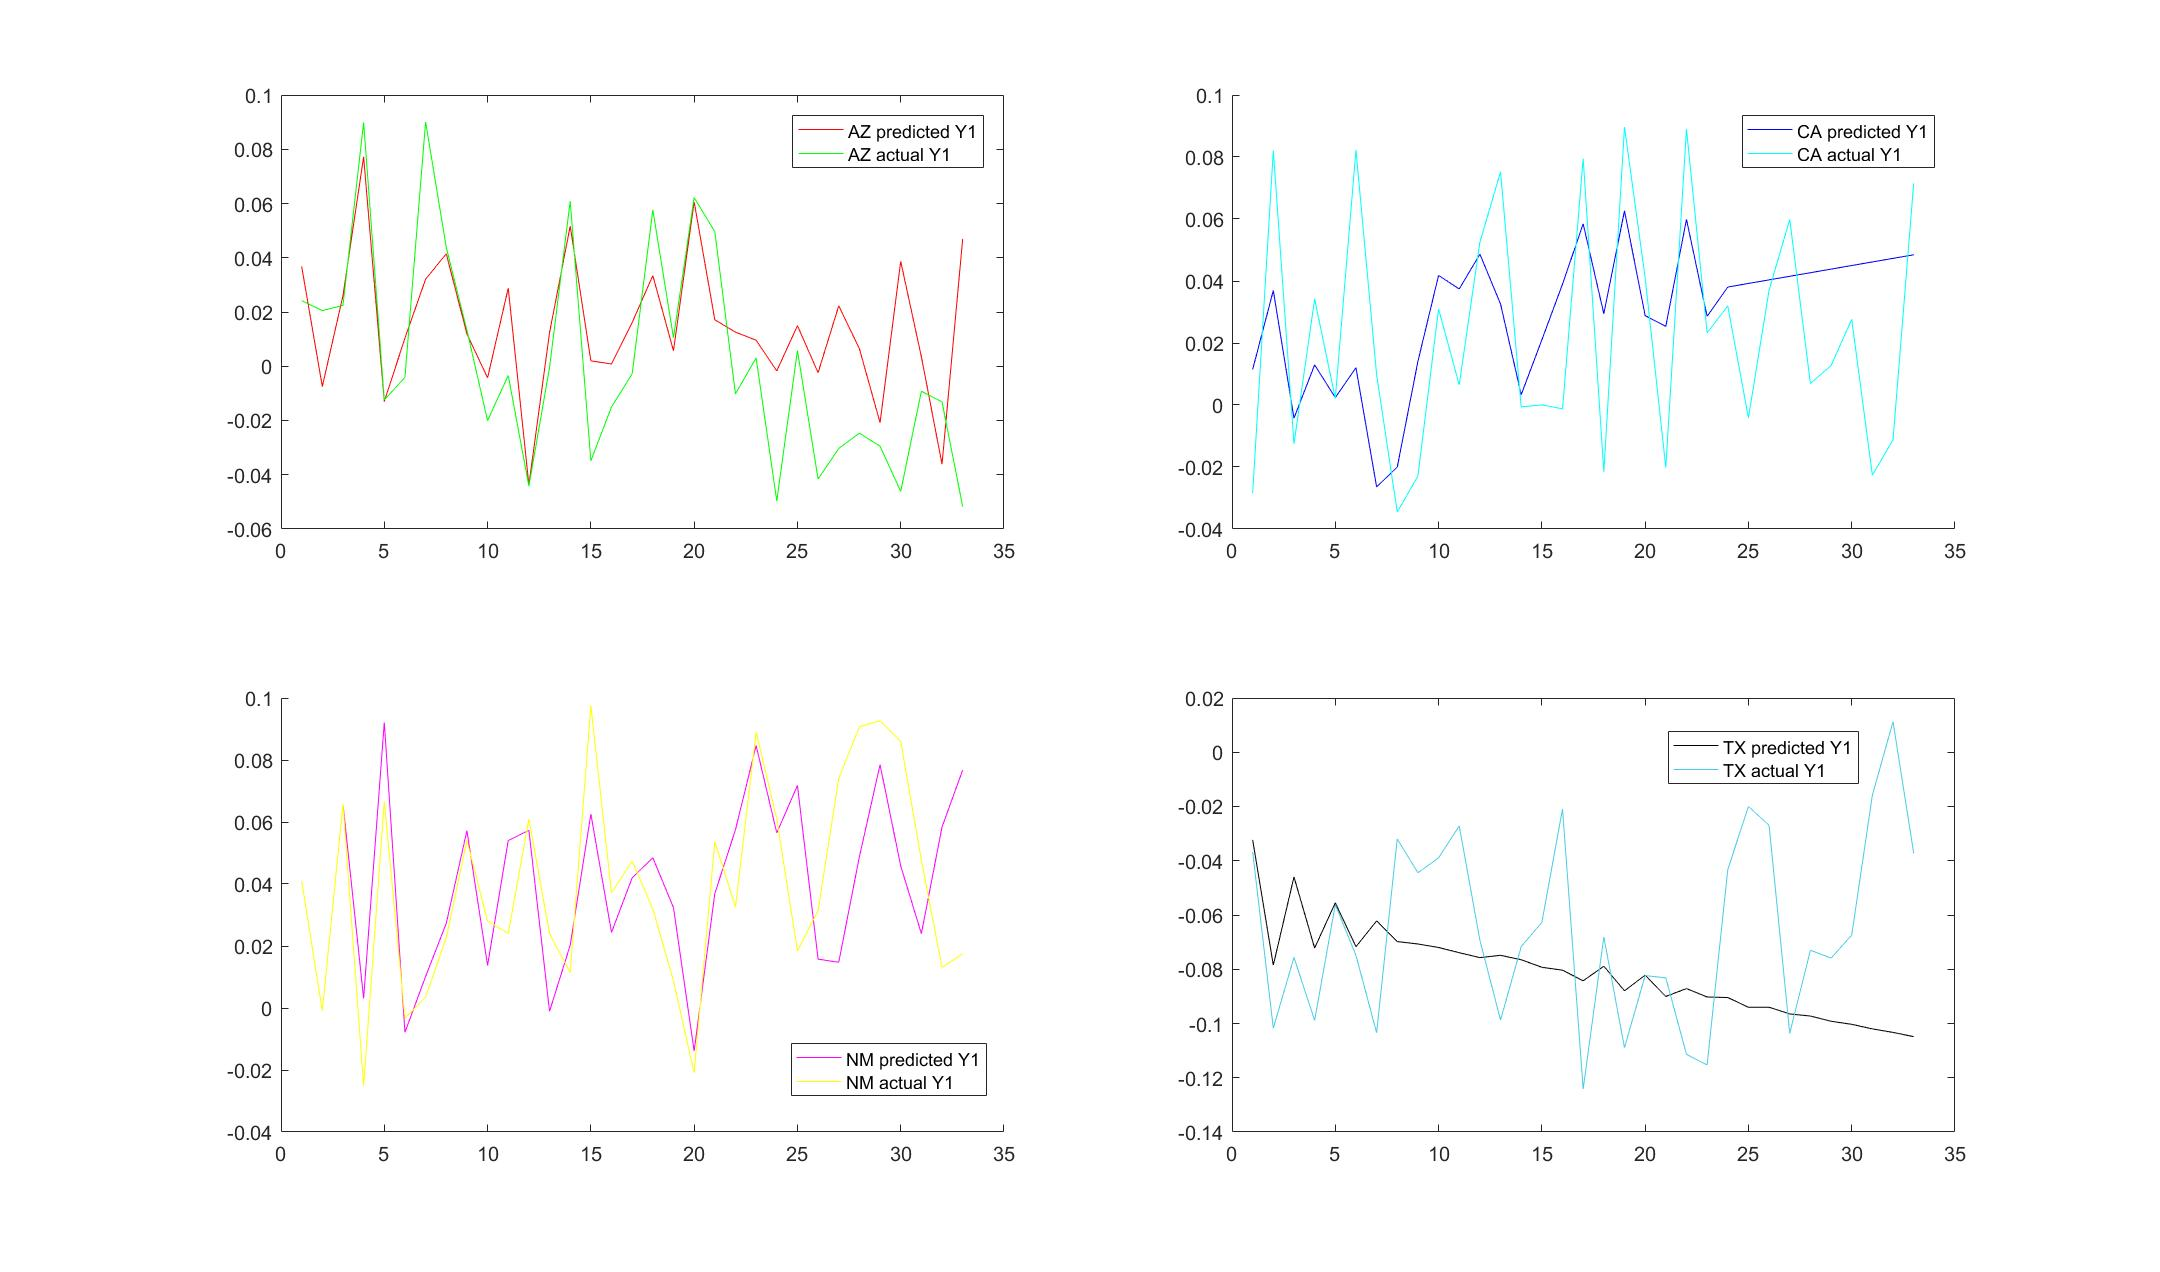
\includegraphics[width=450px]{estimate.jpg}
            \caption{Estimate}
        \end{figure}

    \subsection{Results}

        The model predicts future results as shown below.

        \begin{figure}[!hbpt]
          \centering
          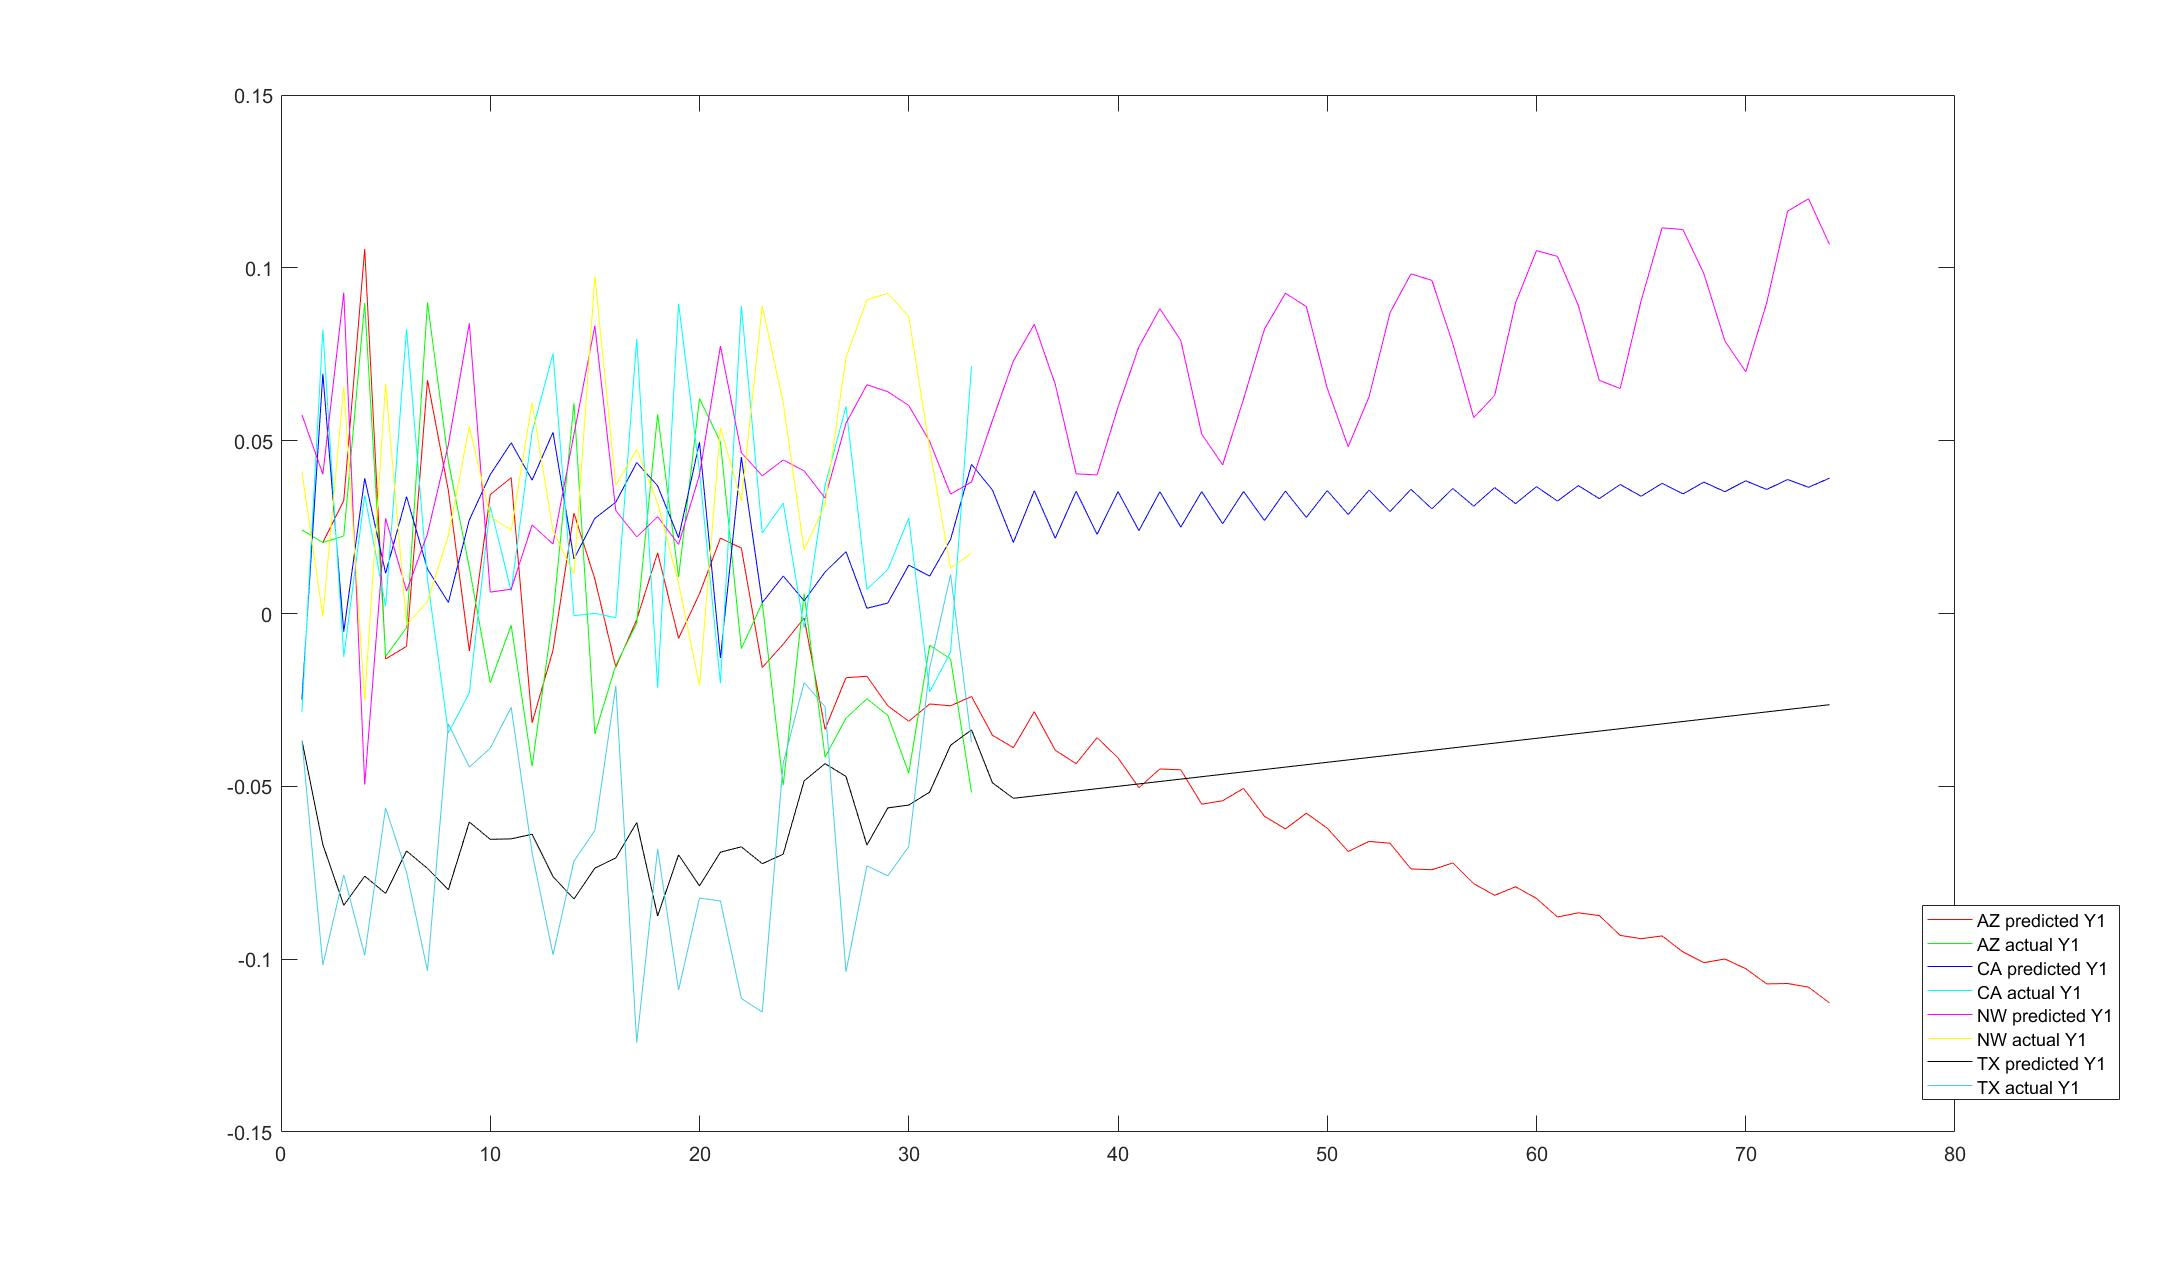
\includegraphics[width=450px]{Y1.jpg}
          \caption{Y1 predition}
        \end{figure}

        \begin{figure}[!hbpt]
          \centering
          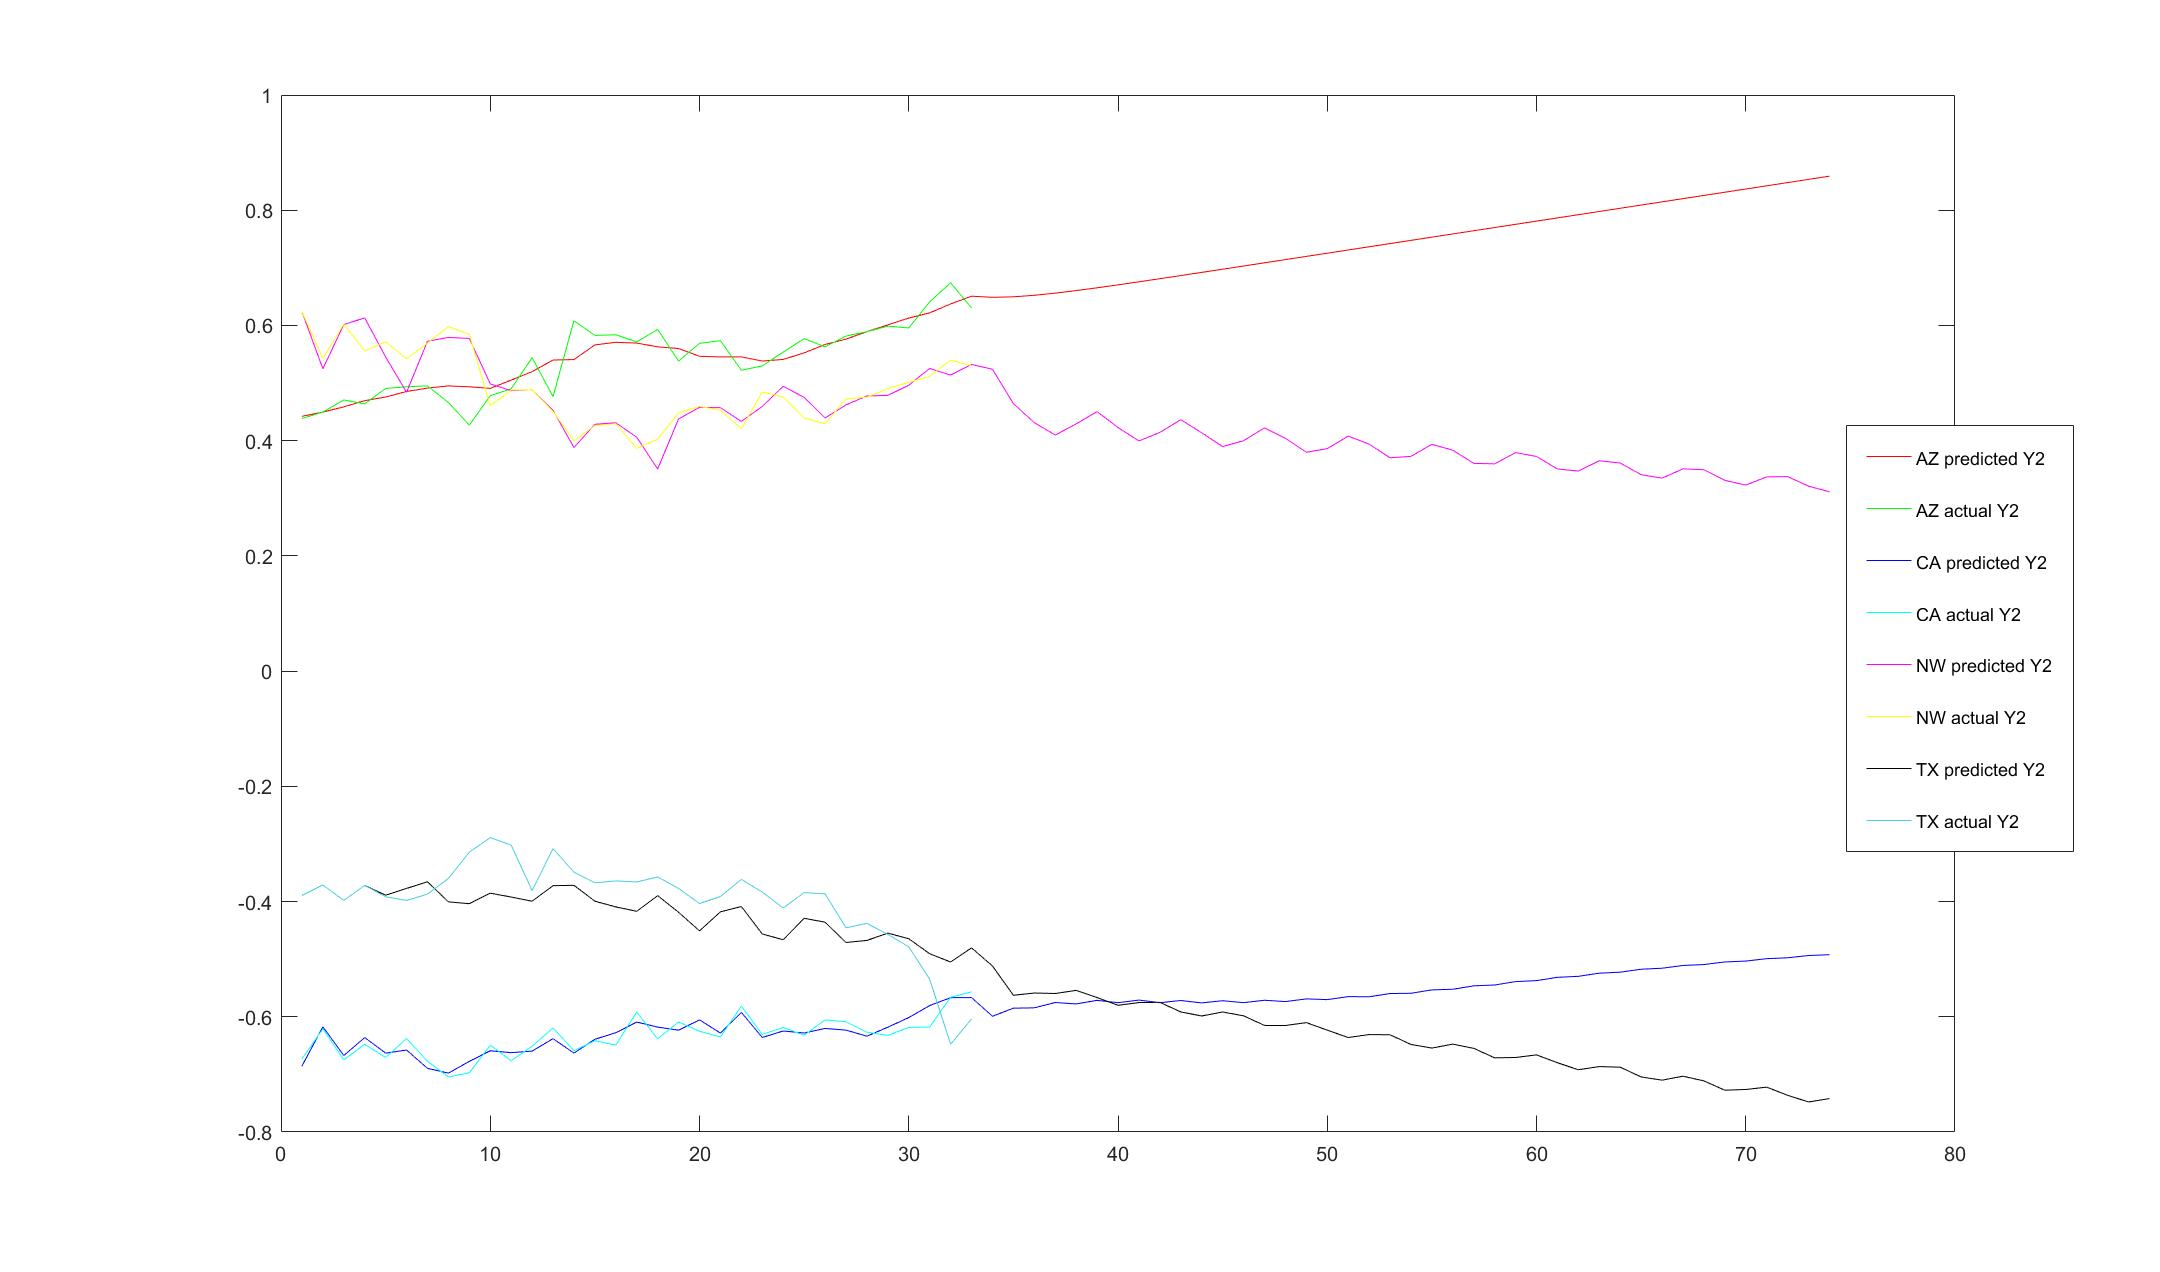
\includegraphics[width=450px]{Y2.jpg}
          \caption{Y2 predition}\label{1}
        \end{figure}

        \begin{figure}[!hbpt]
          \centering
          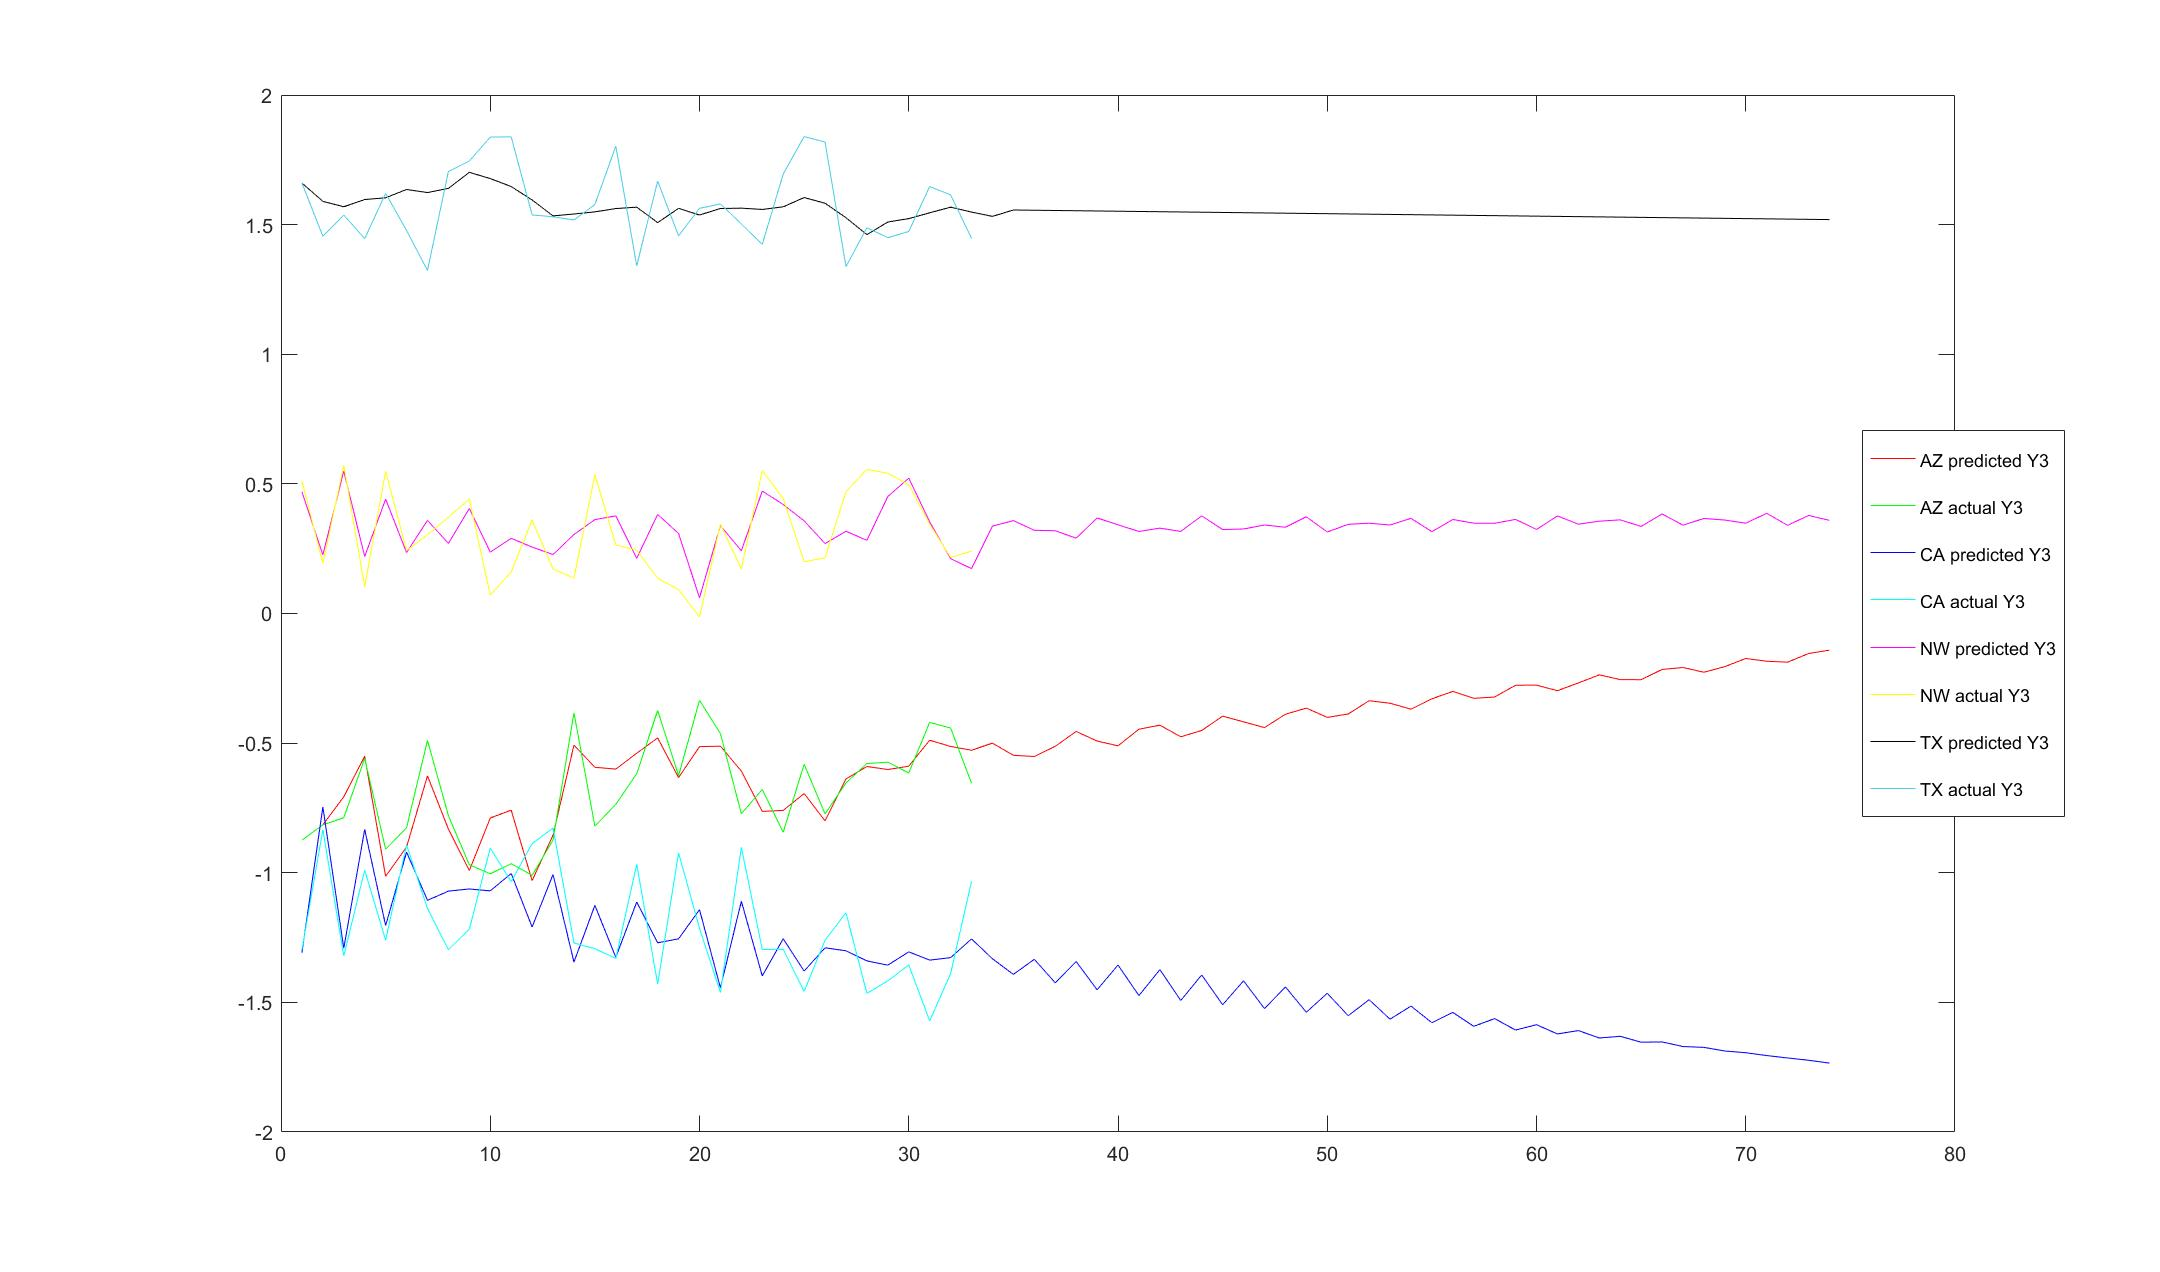
\includegraphics[width=450px]{Y3.jpg}
          \caption{Y3 predition}\label{2}
        \end{figure}


\section{Our suggestions to the governor}
\begin{figure}[h]
%\small
\centering
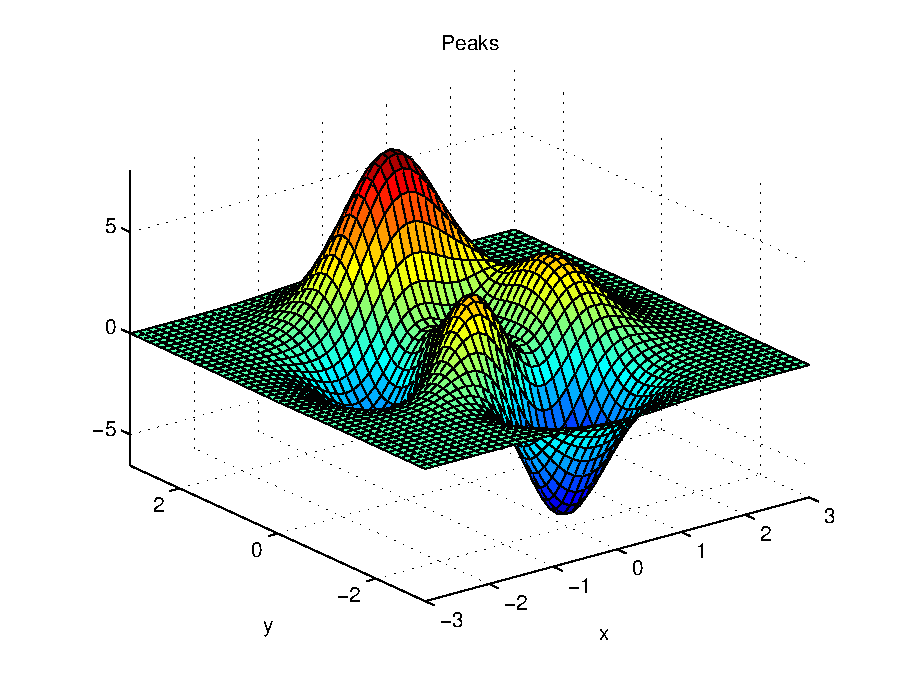
\includegraphics[width=12cm]{mcmthesis-aaa.eps}
\caption{Figure example 1} \label{fig:aa}
\end{figure}


Figure \ref{aa}.

\begin{figure}[h]
\begin{minipage}[h]{0.5\linewidth}
\centering

\includegraphics[width=0.8\textwidth]{0.jpg}
\caption{Figure example 2}
\end{minipage}
\begin{minipage}[h]{0.5\linewidth}
\centering

\includegraphics[width=0.8\textwidth]{0.jpg}
\caption{Figure example 3}
\end{minipage}
\end{figure}



\begin{equation}
a^2 \label{aa}
\end{equation}

\[
  \begin{pmatrix}{*{20}c}
  {a_{11} } & {a_{12} } & {a_{13} }  \\
  {a_{21} } & {a_{22} } & {a_{23} }  \\
  {a_{31} } & {a_{32} } & {a_{33} }  \\
  \end{pmatrix}
  = \frac{{Opposite}}{{Hypotenuse}}\cos ^{ - 1} \theta \arcsin \theta
\]


\[
  p_{j}=\begin{cases} 0,&\text{if $j$ is odd}\\
  r!\,(-1)^{j/2},&\text{if $j$ is even}
  \end{cases}
\]



\[
  \arcsin \theta  =
  \mathop{{\int\!\!\!\!\!\int\!\!\!\!\!\int}\mkern-31.2mu
  \bigodot}\limits_\varphi
  {\mathop {\lim }\limits_{x \to \infty } \frac{{n!}}{{r!\left( {n - r}
  \right)!}}} \eqno (1)
\]

\section{Model analysis}
    \subsection{Sensitivity Analysis}
    \subsection{Strength and weakness}

$\mathop{A}_{ij}$ and $A_{ij}$ 不一样

$\left(123 \right)$ and $(123)$ and (123) 不一样




CTEX中最繁琐的是表格输入,不过数学建模竞赛中,一般要求输入三线表,这样统一格式的情况下,对于输入表格就简单一点了。\\
\\
双斜杠是强制换行,在矩阵,表格,大括号的公式常用。\\
关于表格的合并,见下一部分。给出的例子。
\begin{center}
\begin{tabular}{c|cclcrcc}
\hline
Year & theta & $S_1^-$ & $S_2^-$ & $S_3^-$ & $S_4^+$ & $S_5^+$ & $S_6^+$ \\%表格标题
\hline
2016 & 1      & 0      & 0 & 0.0001 & 0      & 0      & 0 \\
2017 & 0.9997 & 0.0555 & 0 & 0.2889 & 0.1844 & 0.463  & 0 \\
2018 & 0.9994 & 0      & 0 & 0.0012 & 0.3269 & 0.7154 & 0 \\
2019 & 0.9993 & 0      & 0 & 0      & 0.4325 & 1.0473 & 0 \\
2020 & 0.9991 & 0      & 0 & 0      & 0.5046 & 1.2022 & 0 \\
2021 & 0.999  & 0      & 0 & 0      & 0.5466 & 1.2827 & 0 \\
2022 & 0.9989 & 0.0017 & 0 & 0.3159 & 0.562  & 1.2995 & 0 \\
2023 & 0.9989 & 0      & 0 & 0.0109 & 0.5533 & 1.2616 & 0 \\
2024 & 0.9989 & 0      & 0 & 0      & 0.5232 & 1.1769 & 0 \\
2025 & 0.9989 & 0      & 0 & 0.1009 & 0.4738 & 1.0521 & 0 \\
2026 & 0.9991 & 0      & 0 & 0      & 0.4071 & 0.8929 & 0 \\
2027 & 0.9992 & 0.0004 & 0 & 0.1195 & 0.3248 & 0.7042 & 0 \\
2028 & 0.9994 & 0.0164 & 0 & 0.046  & 0.2287 & 0.4902 & 0 \\
2029 & 0.9997 & 0      & 0 & 0.0609 & 0.12   & 0.2545 & 0 \\
2030 & 1      & 0      & 0 & 0      & 0      & 0      & 0 \\
\hline
\end{tabular}
\end{center}

\section{Conclusions}


\begin{center}
\begin{tabular}{c|cc}
\hline
年份 & \multicolumn{2}{c}{指标}\\
\hline
2017 & 0.9997 & 0.0555 \\
2018 & 0.9994 & 0      \\
2019 & 0.9993 & 0      \\
\hline
\end{tabular}
\end{center}


\begin{table}[h]
  \centering
  \begin{tabular}{c|cc}
\hline
年份 & \multicolumn{2}{c}{指标}\\
\hline
2017 & 0.9997 & 0.0555 \\
2018 & 0.9994 & 0      \\
2019 & 0.9993 & 0      \\
\hline
\end{tabular}
  \caption{NAME}\label{SIGN}
\end{table}

Let's to see Table \ref{SIGN}.


\begin{minipage}{0.5\linewidth}
\begin{tabular}{|c|c|c|}
\hline
\multicolumn{2}{|c|}{\multirow{2}{*}{合并}}&测试\\
\cline{3-3}
\multicolumn{2}{|c|}{}& 0.9997  \\
\hline
2019 & 0.9993 & 0 \\
\hline
\end{tabular}
\end{minipage}
\begin{minipage}{0.5\linewidth}
\begin{tabular}{c|ccc}
\hline
年份 & \multicolumn{3}{c}{指标}\\
\hline
\multirow{3}{*}{合并}&2017 & 0.9997 & 0.0555 \\
&2018 & 0.9994 & 0      \\
&2019 & 0.9993 & 0      \\
\hline
\end{tabular}
\end{minipage}






\begin{itemize}
\item \textbf{Applies widely}\\
This  system can be used for many types of airplanes, and it also
solves the interference during  the procedure of the boarding
airplane,as described above we can get to the  optimization
boarding time.We also know that all the service is automate.
\item \textbf{Improve the quality of the airport service}\\
Balancing the cost of the cost and the benefit, it will bring in
more convenient  for airport and passengers.It also saves many
human resources for the airline. \item \textbf{}
\end{itemize}

\begin{thebibliography}{99}
\bibitem{1} D.~E. KNUTH   The \TeX{}book  the American
Mathematical Society and Addison-Wesley
Publishing Company , 1984-1986.
\bibitem{2}Lamport, Leslie,  \LaTeX{}: `` A Document Preparation System '',
Addison-Wesley Publishing Company, 1986.
\bibitem{3}\url{http://www.latexstudio.net/}
\bibitem{4}\url{http://www.chinatex.org/}
\end{thebibliography}

\begin{appendices}

\section{First appendix}



Here are simulation programmes we used in our model as follow.\\

\textbf{\textcolor[rgb]{0.98,0.00,0.00}{Input matlab source:}}
\lstinputlisting[language=Matlab]{./code/mcmthesis-matlab1.m}

\section{Second appendix}

some more text \textcolor[rgb]{0.98,0.00,0.00}{\textbf{Input C++ source:}}
\lstinputlisting[language=C++]{./code/mcmthesis-sudoku.cpp}

\end{appendices}
\end{document}

%%
%% This work consists of these files mcmthesis.dtx,
%%                                   figures/ and
%%                                   code/,
%% and the derived files             mcmthesis.cls,
%%                                   mcmthesis-demo.tex,
%%                                   README,
%%                                   LICENSE,
%%                                   mcmthesis.pdf and
%%                                   mcmthesis-demo.pdf.
%%
%% End of file `mcmthesis-demo.tex'.
